% Manuscript prepared for submission to Empirical Software Engineering
% (Springer). Per EMSE's own submission guidelines
% (https://link.springer.com/journal/10664/submission-guidelines), no
% specific camera-ready LaTeX template is required at initial submission --
% "the compiled PDF will be used for peer-review purposes"; production
% reformats accepted manuscripts. This file therefore uses a generic
% article class but follows EMSE's REQUIRED content structure: title page
% fields, a 150-250 word (optionally structured) abstract, 4-6 keywords,
% author-year in-text citations with an alphabetized DOI-linked reference
% list, an explicit LLM/AI-use disclosure, a Threats to Validity section,
% and a closing Statements and Declarations section.
\documentclass[11pt]{article}
\usepackage[margin=1in]{geometry}
\usepackage{graphicx}
\usepackage{booktabs}
\usepackage{amsmath}
\usepackage[hidelinks]{hyperref}
\usepackage{xcolor}
\usepackage{microtype}
\usepackage[round,authoryear]{natbib}

\title{The Notebook You Read Is Not the Notebook That Ran:\\
Execution-Order Reconstruction for LLM Understanding of Jupyter Notebooks}

% --- Title page fields (EMSE requires: author name(s), affiliation(s),
% corresponding-author email, ORCID if available). Affiliation confirmed by
% the author (Department of Computer Science and Engineering, Rajshahi
% University of Engineering and Technology, Rajshahi, Bangladesh); no ORCID
% will be used. Corresponding-author email confirmed by the author
% (raiyanrohit10@gmail.com). Only the Data Availability Statement's
% repository URL remains a placeholder, pending repo creation.
\author{MD.\ Raiyan Bin Rafique \\
\textit{Department of Computer Science and Engineering} \\
\textit{Rajshahi University of Engineering and Technology, Rajshahi, Bangladesh} \\
Corresponding author: \texttt{raiyanrohit10@gmail.com}}
\date{}

\begin{document}
\maketitle

\begin{abstract}
\noindent\textbf{Context:} Jupyter notebooks store cells in \emph{visual}
order, which routinely diverges from the \emph{execution} order in which they
were actually run, and the serialized JSON buries code under base64 images,
redundant MIME bundles, and metadata. These two defects -- state infidelity
and token bloat -- interact: fixing one tends to worsen the other.
\textbf{Objective:} We ask whether execution-order reconstruction measurably
improves LLM state-tracking accuracy, on both a controlled synthetic
benchmark and real, messy notebooks.
\textbf{Method:} We built JupPreprocessor, a zero-LLM-cost serializer
implementing a three-tier framework (resolve / detect-and-flag /
runtime-verify), evaluated on a fair, context-bounded needle benchmark
across fifteen models/seven vendors, and on executable ground truth from
re-executing 112 real crashed ML notebooks (JunoBench) under both visual and
execution order.
\textbf{Results:} Unaided state-tracking accuracy ranges 0\%--97\% across
adequately-sampled models, while our reordering fix scores 100\% on every
model at $\sim$95\% fewer tokens. On 52 real order-divergent variables,
however, our serializer shows no per-item accuracy advantage over raw JSON
once answered (23--27\% overall-TRUTH, overlapping 95\% CIs) -- a null
result surviving a corrected grading-bug re-analysis. The defensible
real-notebook advantage is narrower: raw JSON overflows context on 62\% of
items versus 15--17\% for compressed serializations.
\textbf{Conclusions:} Execution-order reconstruction is necessary and
sufficient for state-tracking in a fair synthetic setting, but on real
notebooks the serializer is a coverage tool, not yet a demonstrated accuracy
tool.
\end{abstract}

\noindent\textbf{Keywords:} Jupyter notebooks; large language models;
execution-order reconstruction; program state serialization; empirical
software engineering; notebook reproducibility

\section{Introduction}
An LLM asked to debug a Jupyter notebook receives a file that systematically
misrepresents what happened. The \texttt{.ipynb} format records cells in
\emph{visual} order, but users execute, re-execute, reorder, and delete cells
freely; the only trace of the true history is \texttt{execution\_count}
metadata that models demonstrably fail to use reliably
(\S\ref{sec:niah}). Prior work reports ${\sim}36\%$ of GitHub notebooks execute
non-linearly \citep{siddik2025}. We measure the population that actually matters
for LLM assistance -- notebooks saved after \emph{crashed} sessions -- and
find it is far worse: \textbf{59.8\% out-of-order, 89.3\% with re-execution
gaps, 92.0\% with at least one state hazard} (\S\ref{sec:scan}).

Our contributions:
\begin{enumerate}
  \item \textbf{A three-tier treatment framework} distinguishing what a
        serializer can \emph{resolve}, what it can only \emph{detect and flag}
        (because the information is not in the file), and what requires
        \emph{runtime verification}.
  \item \textbf{JupPreprocessor}: a deterministic, zero-LLM-cost serializer
        implementing tiers 1--2, with six static state annotations (mutation
        timelines, ghost last-observed values, divergence-risk flags,
        tolerated/terminal error status, type/shape inference, and an
        execution-order-risk flag for a verified edge case in
        execution\_count-sort itself, affecting 26.6\% of real notebooks)
        at well under 1\% token overhead.
  \item \textbf{A fair Notebook-NIAH benchmark} whose baseline always fits in
        context (overflow is a recorded outcome, never a wrong answer), with a
        compression control, a static/stateful contrast isolating \emph{state
        reconstruction} from \emph{retrieval}, component ablations, and a
        fifteen-model, seven-vendor capability curve.
  \item \textbf{Executable ground truth on real notebooks}: dual-order
        re-execution surfaces real order-divergent variables (``the model you
        think you have is not the model you have''), enabling the first
        real-notebook state-accuracy measurement, including an honest account
        of what remains unsolved.
\end{enumerate}

\section{Root Causes and the Coupling Problem}
\label{sec:causes}
Six state causes afflict \texttt{.ipynb} understanding: (A) non-linear
execution, (B) in-place mutation, (C) ghost variables, (D) re-execution
divergence, (E) silenced errors, (F) type erasure. Four token causes: (G)
redundant MIME bundles, (H) base64-as-text, (I) accumulated outputs, (J) JSON
nesting overhead. They couple: restoring state costs tokens; cutting tokens
strips state.

\textbf{Three of the six state causes are information-theoretically unsolvable
from a cold \texttt{.ipynb}.} Post-mutation values (B), ghost origins (C), and
output drift (D) are not stored in the file. This dictates the framework of
Table~\ref{tab:tiers}. The tier-2 insight: the LLM does not need the missing
value to avoid errors -- it needs to know \emph{that} it is missing and
\emph{where} uncertainty was introduced. A flagged unknown prevents confident
wrong reasoning; a silent unknown invites it.

\begin{table}[t]
\centering\small
\begin{tabular}{@{}lllp{6.2cm}@{}}
\toprule
Tier & Treatment & Causes & Mechanism \\
\midrule
1 & Resolve & A, G--J & Reorder by \texttt{execution\_count}; strip
MIME/base64/metadata; latest output only; YAML \\
2 & Detect \& flag & B--F & Mutation timeline; ghost last-observed value;
divergence-risk flags; tolerated/terminal errors; typed shape hints \\
3 & Runtime verify & B--E fully & Sandboxed re-execution diffed against static
predictions \\
\bottomrule
\end{tabular}
\caption{The three-tier treatment framework.}
\label{tab:tiers}
\end{table}

\section{JupPreprocessor}
\label{sec:method}
A single-pass, deterministic Python transform; no LLM, no network, no kernel.
Output: YAML with \texttt{execution\_order}, chronologically sorted cells
(markdown re-associated with the executed cell it precedes), per-cell
annotations (\texttt{error\_status}, \texttt{divergence\_risk}), and a
\texttt{variables} table (type, shape, defined\_in, last\_modified, history,
status $\in$ \{active, ghost\}, confidence). Cells the AST rejects (IPython
magics, shell escapes) degrade to regex extraction rather than failing the
notebook.

\subsection{Use of large language models and AI agents in this study}
\label{sec:llmuse}
Per this journal's authorship policy, we document LLM/AI-tool use explicitly
rather than treating it as incidental. LLMs are used in two structurally
different roles in this work, and we distinguish them throughout: (1) as
\emph{answer models under test} in the evaluations themselves (e.g.\ the
fifteen models on the synthetic benchmark, gpt-4o on the real-notebook
evaluation) -- this is the object of study, not a tool used to produce the
study; and (2) as \emph{research and drafting assistance}, specifically: an
automated grading judge (gpt-4o-mini) used to classify free-text answers
against stored ground-truth candidates on the real-notebook evaluation
(\S\ref{sec:realnb}), whose reliability we independently audited and whose
discovered bug we report in full (\S\ref{sec:judgeaudit}) rather than
treating as incidental tooling; and an LLM-based coding/research agent used
throughout the project to write experiment scripts, run the reported
measurements, draft prose from the resulting reports, and perform an
independent verification pass cross-checking every quantitative claim in this
manuscript against its underlying source report or script output (the
verification log is retained in the project repository; see the Data
Availability statement). No LLM is credited as an author, consistent with
this journal's position that LLMs do not satisfy authorship criteria; the
corresponding author takes full accountability for the accuracy of all
claims, having directed and reviewed every experiment and correction
described in this manuscript, including the several instances (the judge
bug, the \texttt{execution\_count}-sort edge case, and the Themisto
explanation) where an initial LLM-assisted result was subsequently found to
be wrong and was corrected rather than published as-is.

\section{Experimental Design Principles}
(1)~\textbf{Fairness}: any prompt exceeding the context cap is a recorded
\textsc{overflow}, never an ``incorrect''; a baseline may only fail by
answering wrong \emph{while fitting}. (2)~\textbf{Controls}:
\texttt{plain\_strip} (same compression, visual order, no table) separates
compression from structure; \texttt{reorder\_only} / \texttt{table\_only}
ablate components. (3)~\textbf{Static vs.\ stateful contrast}: identical
needle string; only the stateful mode reassigns it out of order behind a
visually-later decoy. (4)~\textbf{Determinism}: CRC32-seeded haystacks; seeded
RNGs in dual-order re-execution. (5)~\textbf{Honest reporting}: negative
results and by-construction caveats stated alongside the results that carry
them.

\section{Results}

\subsection{Compression and robustness on real notebooks}
On 40 real crashed ML notebooks (JunoBench \citep{wang2025junobench}, seed 42):
\textbf{40/40 preprocessed without error; 96.4\% aggregate / 91.2\% median
token reduction} (largest single case 7.5M $\to$ 11.2k tokens; one
already-lean notebook \emph{grew} 2.3\% -- the ``already-clean'' failure
mode, quantified at 1-in-40). All six state annotations together (the
original five B--F flags plus the \texttt{execution\_order\_risk}
annotation described in \S\ref{sec:threats}) cost well under 1\% extra
tokens (Figure~\ref{fig:tokens}); median reduction moved from 91.5\% to
91.2\% when the sixth annotation was added.

\begin{figure}[t]
\centering
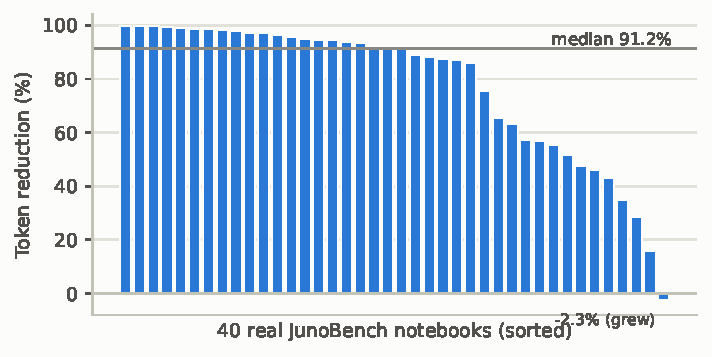
\includegraphics[width=.85\linewidth]{figures/fig2_token_reduction.pdf}
\caption{Per-notebook token reduction on 40 real JunoBench notebooks, sorted.
The single negative case is an already-lean notebook that grows under YAML plus
the state table.}
\label{fig:tokens}
\end{figure}

\subsection{Fair Notebook-NIAH: retrieval is not the failure mode; state is}
\label{sec:niah}
Depths $\{0.1, 0.5, 0.9\}$ $\times$ lengths $\{8\text{k}, 30\text{k},
60\text{k}, 100\text{k}\}$ tokens, all under a 126k cap; 3 trials/cell (the
two 2026-03 snapshots: 1 trial/cell). \textbf{Static mode} (gpt-4o): 100\% for
all conditions at every grid cell (depth $\times$ length) -- noise alone does
not impair retrieval when context fits, correcting a common overclaim. \textbf{Stateful mode} across
fifteen models (nine OpenAI on the full 36-trial grid, plus six non-OpenAI
models -- NVIDIA Nemotron-3-Super-120B, MiniMax-M3, Cohere
North-Mini-Code, InclusionAI Ling-3.0-Flash-Fin, Poolside Laguna-S-2.1, and
Zhipu GLM-5.3-Flash -- on a reduced grid: 1 length $\times$ 3 depths
$\times$ 1--2 trials $\times$ 3 conditions, to fit each provider's free-tier
rate limit) is shown in Figure~\ref{fig:curve}: \texttt{raw} ranges 0\%
(MiniMax-M3, Cohere North-Mini-Code) to 97\% (gpt-5, full grid) -- GLM-5.3-Flash
scored 100\% unaided on only $n=3$ trials, too thin to treat as a reliable
ceiling; \texttt{plain\_strip} ${\approx}0\%$
everywhere; \texttt{ours} \textbf{100\% on every model}. Ablations (gpt-4o):
\texttt{reorder\_only} 100\%, \texttt{table\_only} 0\%.

Five readings. (i)~Out-of-order reassignment degrades every model even though
the resolving metadata is present in the JSON; failures concentrate at deep
positions. (ii)~\textbf{Three generations of OpenAI model scaling took unaided state
resolution from 3\% to 97\% without closing the gap a deterministic serializer
closes completely on every model} -- at ${\sim}95\%$ fewer tokens.
(iii)~Compression does not help and metadata cannot substitute for reordering:
\textbf{execution-order reconstruction is necessary and sufficient}.
(iv)~Neither tiers nor generations are monotonic (gpt-4.1-nano $>$
gpt-4.1-mini; the 2026-03 gpt-5.4-mini scores below the earlier gpt-5-mini),
so serialization is a more reliable lever than model choice.
(v)~\textbf{The six non-OpenAI models mostly replicate the pattern, with one exception}: MiniMax-M3's and
Cohere North-Mini-Code's raw scores (0\%) are tied for the single worst in the entire curve,
Nemotron-3-Super's (50\%) lands mid-pack, InclusionAI Ling-3.0-Flash-Fin (33\%) and
Poolside Laguna-S-2.1 (67\%) fall between them, and GLM-5.3-Flash uniquely scored
100\% raw on its $n=3$ sample -- all six are fixed completely by \texttt{ours} regardless. With
$n=3$--$6$ trials per non-OpenAI model on a reduced grid, this is a spot check, not a demonstration of
broad cross-vendor generality; it supports only that five of the six additional
vendors checked did not contradict the pattern, and the sixth (GLM-5.3-Flash) is too
thinly sampled to draw a conclusion from either way. We note the
\texttt{ours} 100\% is partly by-construction -- the benchmark instantiates
the exact defect the tool fixes; the load-bearing findings are the raw
capability curve and the controls.

\begin{figure}[t]
\centering
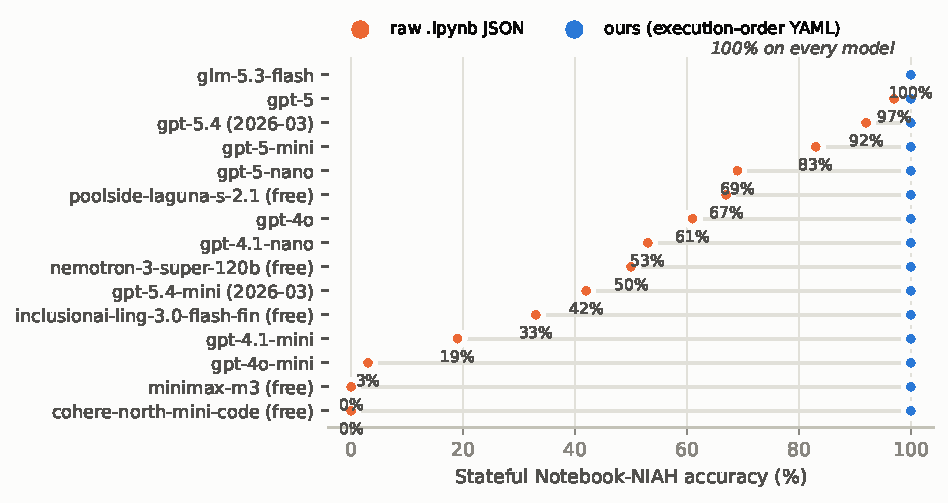
\includegraphics[width=.9\linewidth]{figures/fig1_model_curve.pdf}
\caption{Stateful Notebook-NIAH accuracy across fifteen models: nine OpenAI
models spanning four generations, plus six non-OpenAI models (NVIDIA
Nemotron-3-Super-120B, MiniMax-M3, Cohere North-Mini-Code, InclusionAI
Ling-3.0-Flash-Fin, Poolside Laguna-S-2.1, Zhipu GLM-5.3-Flash) on a reduced
grid, each via its own free tier. Unaided (\texttt{raw}) accuracy spans 0\% to 97\%
on every adequately-sampled (full-grid) model and never reaches the 100\% that
execution-order reconstruction (\texttt{ours}) achieves on every model; one
thinly-sampled exception (GLM-5.3-Flash, $n=3$) also scored 100\% raw, too
small a sample to draw a conclusion from. \texttt{plain\_strip} (not shown) is ${\approx}0\%$
throughout.}
\label{fig:curve}
\end{figure}

\subsection{State hazards are the norm in the debugging population}
\label{sec:scan}
Across all 112 original JunoBench notebooks: \textbf{59.8\% non-monotonic}
(visual $\neq$ execution order), \textbf{89.3\% with execution-count gaps}
(re-execution or deleted cells -- the ghost precondition), \textbf{92.0\%
with at least one hazard}. Against the ${\sim}36\%$ GitHub-wide
figure \citep{siddik2025}: the notebooks most likely to be handed to an LLM are
the most misleading.

\subsection{Executable ground truth on real notebooks}
\label{sec:realnb}
Each out-of-order notebook is executed twice in an isolated sandbox (per-cell
timeouts, identical seeds): once in \texttt{execution\_count} order, once in
visual order. Initially with \texttt{torch}/\texttt{torchvision} installed
(CPU wheels; Python 3.14), and later widened using a dedicated Python 3.12
virtual environment with TensorFlow (\texttt{tensorflow} has no Python-3.14
wheel at time of writing), 62/67 executed usefully; \textbf{16 notebooks
yield 52 order-divergent variables} -- a conservative lower bound (many
notebooks still could not fully execute for lack of data files and heavy
dependencies; one TensorFlow notebook remains unexecutable due to a large
mid-execution network download racing a per-cell timeout, a genuine
flaky-network case rather than a missing-dependency case; run-to-run
variance of 52--55 items was observed across repeated extraction runs, traced
to network-dependent notebook code). Two
kinds: \emph{value divergence} (in \texttt{sklearn\_9}, the final model is
\texttt{LogisticRegression()} in truth but
\texttt{LogisticRegression(solver='liblinear')} under visual reading) and
\emph{existence divergence}, introducing \textbf{phantom variables} -- the
mirror image of ghosts: visible in the file, never survived the session.

LLM evaluation on all 52 items (gpt-4o; three-way judge: \textsc{truth} =
execution-order state, \textsc{decoy} = visual-order state) appears in
Figure~\ref{fig:realstate}, \emph{after fixing a judge bug found by manual
audit} (below), with 95\% Wilson intervals on the overall-truth rate: raw
23\% [14,36], plain\_strip 27\% [17,40], ours 27\% [17,40]. Four findings,
reported through three rounds of self-correction. \textbf{Access is the robust
finding, unchanged by any correction and if anything strengthening}: raw JSON overflows context on
62\% of real divergent items at $n{=}52$ (up from 51\% at $n{=}41$, since
larger real notebooks kept entering the corpus); ours
reaches 85\% and plain\_strip 83\%. \textbf{Accuracy-when-answered shows no
distinguishable advantage for ours, replicated at larger $n$}: ours and
plain\_strip are
tied at 27\% overall-\textsc{truth}, raw trails nominally at 23\%,
and all three intervals overlap heavily -- the same conclusion as the
$n{=}41$ post-judge-fix result, now confirmed rather than reversed by more
data. \textbf{The correction history is
itself a finding.} A 13-item pilot suggested a clean win (6/13 vs.\ raw's
3/13). Expanding to 41 items narrowed this to statistical noise. A manual
audit of the automated gpt-4o-mini judge (25-item independent re-check,
\S\ref{sec:judgeaudit}) then found a 24\% disagreement rate concentrated in
one mechanism: whenever a ground-truth candidate was ``never defined,'' the
judge tended to credit any concrete answer to the \emph{other} candidate
without verifying the value matched -- a bug that happened to reward ours's
tendency to produce confident (sometimes wrong) guesses from its variable
table. Fixing the judge prompt to require literal/close value matches removed
ours's apparent edge entirely. Expanding the corpus again to 52 items (via
the Python 3.12/TensorFlow environment) reproduced the corrected null result
rather than reversing it. We report all four stages because each
successive correction moved the conclusion in the same (more modest)
direction or replicated it.

\subsection{Judge validation}
\label{sec:judgeaudit}
An independent second-pass re-grading (not a human-subjects study; the
reviewing agent manually compared each sampled answer against the stored
ground-truth candidates without invoking an LLM classifier) on 25 of 123
answer rows found 19/25 (76\%) agreement with the original automated judge.
All 6 disagreements shared one mechanism, confirmed with a reproducible
example: for \texttt{numpy\_1.ipynb}'s \texttt{device} (truth = never
defined, decoy = \texttt{cpu}), the identical answer content (\texttt{cuda})
was graded \textsc{decoy} in one condition and \textsc{truth} in another --
neither is correct, since \texttt{cuda} matches neither candidate literally.
The judge prompt was rewritten to require an explicit literal/close value
match and to default to \textsc{neither} on uncertainty; full untruncated
answers are now persisted for future audits
(\texttt{tests/real\_state\_eval\_raw\_answers.json}). Full detail in
\texttt{reports/judge\_validation\_report.md}.

\begin{figure}[t]
\centering
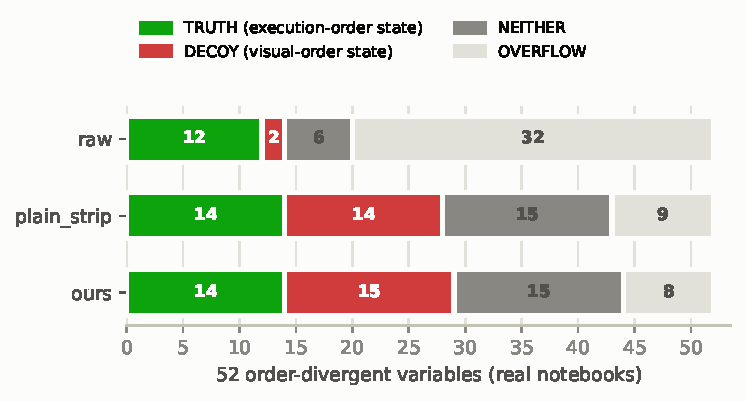
\includegraphics[width=.85\linewidth]{figures/fig3_real_state_outcomes.pdf}
\caption{Outcomes on the 52 real order-divergent variables per serialization.
\textsc{overflow} = the prompt could not fit the 126k context cap.}
\label{fig:realstate}
\end{figure}

\subsection{Honest negatives}
On the pre-cleaned Themisto dataset \citep{grotov2025themisto}, preprocessing
\emph{reduced} output-prediction accuracy (40.0\% $\to$ 26.7\%) and added
token overhead. A follow-up measured breakdown (not inferred) found the
published explanation for this was wrong: of the items where \texttt{ours}
is wrong, most (9/11) are \emph{also} wrong under raw -- both formats
guessing on data neither has access to -- and only 2 of 15 items decide
the entire gap. In both decisive items the correct value was present
verbatim in the preprocessed prompt; it was not stripped or lost. What
actually differs, measured directly: the variable-state table sits between
the code/output history and the query, pushing the correct evidence
2.7--7.7$\times$ farther (by character distance) from the point of
prediction than in the raw format, and the model's wrong answers matched a
closer-but-incorrect earlier value in both cases -- a lost-in-the-middle /
distraction effect, not an information-loss effect. Structure is a net
negative specifically when there is no token bloat to justify the added
distance to the query. On JunoBench debugging with full
context, accuracy was identical (8/8 both) with 79.1\% token savings -- a
cost result, not an accuracy result.

\section{Threats to Validity}
\label{sec:threats}

\subsection{Construct validity}
The Notebook-NIAH synthetic benchmark is, by construction, favorable to our
method: it instantiates exactly the defect (out-of-order reassignment) our
pipeline is designed to fix, so a perfect \texttt{ours} score demonstrates
the transform is correct and complete for that defect, not that language
models generally prefer our output format. We treat its controls
(\texttt{plain\_strip}, \texttt{reorder\_only}, \texttt{table\_only}) and the
independent real-notebook study, rather than the \texttt{ours}~=~100\%
figure in isolation, as the load-bearing evidence. The automated LLM judge
used for real-notebook grading (gpt-4o-mini) had a measured 24\% disagreement
rate with independent manual re-grading before a discovered bug was fixed
(\S\ref{sec:judgeaudit}); readers should treat exact TRUTH/DECOY counts as
approximate even after the fix, since no fully human-annotated ground truth
exists for this task. \texttt{execution\_count}-sort itself has a real,
verified construct-validity issue: \texttt{execution\_count} records only a
cell's \emph{last} run, not a mutually-consistent history, so a re-run early
cell (e.g.\ an import, after a kernel restart) can sort after code that
already uses it -- a sequence not runnable in a fresh kernel and not
corresponding to any real moment in the notebook's history. Verified in
\texttt{numpy\_1.ipynb} (import cell $\texttt{execution\_count}{=}27$, a cell
needing \texttt{torch} $\texttt{execution\_count}{=}2$; see
\texttt{reports/execution\_count\_reordering\_limitation.md}), where the
\texttt{execution\_order\_risk} annotation verifiably fires on exactly 6
affected cells. An earlier, smaller snapshot of the ground-truth corpus
($n{=}41$, before the Python 3.12/TensorFlow expansion to $n{=}52$)
estimated this mechanism plausibly explained 8 of those 41 items (7 from
\texttt{numpy\_1.ipynb}, 1 from \texttt{torch\_4.ipynb}) rather than genuine
out-of-order-execution divergence; we have not re-quantified this specific
estimate at $n{=}52$, and flag it as an estimate from an earlier corpus
snapshot rather than a current, re-verified count. Both \texttt{ours} and
the ground-truth methodology inherit the underlying assumption regardless.
A follow-up corpus-wide static scan
($\$0$, no LLM calls; \texttt{reports/execution\_count\_consistency\_report.md}),
restricted to import-bound names for a cleaner signal than a noisier broad
count dominated by legitimate reuse of generic identifiers, finds this
affects \textbf{29 of 109 analyzable JunoBench notebooks (26.6\%)} --
common enough to fix. The preprocessor now detects and flags it: a new
\texttt{execution\_order\_risk} per-cell annotation, verified to fire on
exactly the 6 affected cells in \texttt{numpy\_1.ipynb}, passing all
existing unit tests, at negligible token cost. Detect-and-flag was chosen
over a hybrid reordering fix as the lower-risk option, consistent with the
paper's own three-tier philosophy of flagging unresolvable uncertainty
rather than guessing.

A related hypothesis --- that environment-dependent branching (e.g.\
\texttt{torch.cuda.is\_available()}-style checks, whose outcome depends on
the runtime environment rather than anything visible in the file) is a
static-analysis blind spot \emph{distinct} from the \texttt{execution\_count}-sort
edge case above --- was tested directly against the $n{=}41$ ground truth
rather than left as an untested inference, and the result is genuinely
inconclusive rather than confirmatory. 8 of 41 items matched an
environment-branching regex, with a striking raw correlation (88.2\% wrong
answers vs.\ 48.1\% for non-flagged items); however, all 8 flagged items
share the identical \texttt{phantom\_in\_visual}/\texttt{ec\_order\_value=None}
signature already explained by the \texttt{execution\_count}-sort mechanism,
so this corpus contains zero cases separable from that confound. We report
this as an honest null/inconclusive result --- not evidence the hypothesis
is false, but evidence that this specific corpus cannot test it --- rather
than omitting a tested-but-inconclusive hypothesis from the record.
(\texttt{reports/environment\_branching\_check.md})

\subsection{Internal validity}
At $n{=}52$, after fixing an identified judge bug and replicating at
$13\to41\to52$ items, \texttt{ours} shows \emph{no} accuracy-when-answered
advantage over \texttt{raw} or a plain compression control
(\texttt{plain\_strip}) -- \texttt{ours} and \texttt{plain\_strip} are tied
at 27\%, \texttt{raw} trails nominally at 23\%, all within noise. The
real-notebook claim this paper stands behind rests entirely on
reach/coverage, not on any demonstrated per-item accuracy advantage of
structure over compression -- a further downgrade from an earlier,
already-downgraded 13-item and then 41-item pre-fix draft, now replicated
(not reversed) at 52 items, reported transparently as such. We did not
attempt a formal power analysis before concluding this is a genuine null
result rather than an underpowered one; at the observed effect sizes, a
substantially larger item count (plausibly 150+) would be needed to resolve
this with confidence, and we flag this explicitly as an open question rather
than treating $n{=}52$ as decisive. Real-notebook state accuracy is a 52-item
case study (the full population recoverable across a Python 3.14 environment
with torch/torchvision and a separate Python 3.12 environment with
TensorFlow, not a random sample); one TensorFlow notebook remains
unexecutable due to a flaky, timeout-sensitive network download rather than
a missing dependency, and run-to-run item-count variance of 52--55 was
observed due to genuine network-dependent notebook code. Static extraction
cannot mark runtime failure of visible code (phantoms) -- measured as the
dominant remaining error class regardless of serialization condition.

\subsection{External validity}
Fifteen answer models total on the synthetic stateful benchmark; nine are
OpenAI, and six (NVIDIA Nemotron-3-Super-120B, MiniMax-M3, Cohere
North-Mini-Code, InclusionAI Ling-3.0-Flash-Fin, Poolside Laguna-S-2.1, Zhipu
GLM-5.3-Flash, each via its own free tier) are non-OpenAI, on a reduced grid
(1 length $\times$ 3 depths $\times$ 1--2 trials $\times$ 3 conditions) to fit
each provider's rate limit. \texttt{ours} is 100\% on all six regardless;
five of the six replicate the qualitative pattern of imperfect, non-monotonic
\texttt{raw} accuracy, while the sixth (GLM-5.3-Flash) scored 100\% raw on
only $n{=}3$ trials. This is reassuring but $n{=}3$--$6$ per model is not a
broad cross-vendor sample -- it supports only that most of the six
additional vendors checked did not contradict the pattern, not general
cross-vendor independence, and the one exception is too thinly sampled to
interpret either way. Two free-tier candidates (Google Gemma-4-31B, NVIDIA
Nemotron-3-Ultra-550B) and a Gemini 3.7/3.8 Flash attempt were dropped after
confirmed persistent upstream unavailability (exhausted retries, or -- for
Gemini specifically -- repeated HTTP 400/503 errors traced to free-tier
capacity limits, confirmed reproducible with two independent API keys and
therefore not our account), consistent with this project's standing policy
of dropping rather than fighting confirmed-flaky providers rather than
reporting an unreliable data point. The real-notebook evaluation used gpt-4o
exclusively. All real-notebook data is drawn from a single benchmark corpus
(JunoBench); generalization to notebooks outside this crashed-ML-notebook
population is untested. On the cost of Tier 3 (runtime verification, \S2):
our framing already restricts it to ``when a kernel is permissible,'' and
external evidence supports that restriction rather than suggesting it is
overly conservative. A 2026 preprint (FlowBook) reports lightweight dynamic
instrumentation at a median 70ms/cell overhead -- cheap, but only \emph{while
a notebook is already executing}; it is not a way to validate one isolated
cell without a kernel, so it does not relax our no-kernel constraint for
Stage 1, only suggests Tier 3 is less costly than assumed in contexts (e.g.\
an interactive agent session) where a kernel is already attached for other
reasons.

\section{Related Work}
Notebook agents and stateful runtimes -- DatawiseAgent \citep{you2025datawise},
CaveAgent \citep{ran2026caveagent}, DeltaBox \citep{dong2026deltabox}, I-PTC
\citep{gonzalez2026} -- assume a live kernel; serialization-side tooling is
either lossy (Jupytext \citep{jupytext}, notebookllm \citep{notebookllm} strip
outputs) or unevaluated base64 stripping. Benchmarks --
Themisto \citep{grotov2025themisto}, JunoBench \citep{wang2025junobench},
NbQA/Jupiter \citep{li2025jupiter}, DABStep \citep{egg2025dabstep} -- test
tasks, not serializations; none isolate execution-order reconstruction. To
our knowledge no prior work measures LLM state accuracy against dual-order
executable ground truth on real notebooks.

The closest prior art is \textbf{CRABS} \citep{li2025crabs} (COLM 2025), which
reconstructs a notebook's execution-dependency graph via static/syntactic
analysis plus an LLM disambiguation step, reporting 98--99\% F1 on 50 real
Kaggle notebooks. This is meaningful validation that a static-analysis-plus-LLM
approach class can recover notebook execution structure without
re-execution -- but CRABS's accuracy depends on its LLM step, making it
closer to our optional Stage 2 than to our zero-LLM-cost Stage 1 in
isolation, and its evaluation sample (``highly-upvoted'' Kaggle notebooks) is
markedly cleaner than the crashed, messy corpus we study; we do not know
whether CRABS's accuracy transfers to that harder setting. Two 2026
benchmarks independently corroborate that state-tracking during
notebook-style analysis remains an open capability gap for current models,
beyond the older reproducibility literature we already cite:
\textbf{LongDS-Bench} \citep{xu2026longds} finds the best model reaches only
48.45\% accuracy on maintaining/restoring analytical state across
long-horizon, real-Kaggle-notebook-derived tasks (a ${\sim}47$-point accuracy
drop from early to late turns, with the authors attributing the bottleneck to
state maintenance rather than interaction budget), and
\textbf{DSAgentBench} \citep{rahman2026dsagentbench} finds the best model succeeds on
only 56.70\% of 275 real, full-environment data-science tasks. Neither
targets serialization directly, but both strengthen the motivating claim that
this problem is unsolved at the agent level, not merely a
reproducibility-literature curiosity.

A structurally different alternative is \textbf{reactive/dataflow notebooks
(marimo)} \citep{marimo}, which eliminate hidden state and out-of-order execution
\emph{by construction} rather than by post-hoc reconstruction, at the cost
of requiring conversion away from \texttt{.ipynb}. We tested marimo's
official conversion tooling (\texttt{marimo convert} + \texttt{marimo export
html}) on the same 40-notebook real, crashed corpus used in \S5.1:
conversion and reactive execution never crashed or timed out
(\textbf{40/40 tooling-reliable}), but \textbf{every single notebook (40/40)
had at least one cell fail during execution}, almost always from missing
local data files or third-party packages absent from the runtime environment
-- the identical ``missing deps/data'' failure mode our own dual-order
re-execution ground truth already reports for these notebooks. This is
evidence \emph{for}, not against, a static, execution-free approach on the
specific axis of \emph{reach}: any method requiring live execution, marimo's
reactive model included, inherits the real-world unavailability of a
notebook's original data/environment, while a purely static method cannot be
blocked by a missing package or file since it never attempts to run
anything. We did not compare marimo's recovered variable states against our
executable ground truth where both approaches \emph{can} execute; that
remains open. (\texttt{reports/marimo\_conversion\_report.md})

\section{Conclusion}
Two defects, one mechanism: strip what the file wastes, reconstruct what it
scrambles, and \emph{say what it cannot know}. Execution-order reconstruction
is necessary and sufficient for the measurable state failure in a fair
synthetic setting, at $\sim$95\% fewer tokens and effectively zero inference-time
cost. That result does \emph{not} cleanly transfer to real notebooks as an
accuracy advantage: on 52 real order-divergent variables, \texttt{ours} and a
plain compression control are tied and \texttt{raw} trails, all within
statistical noise once an answer is reached -- a conclusion that replicated,
rather than reversed, when we expanded the corpus from 41 to 52 items. What
transfers, and what we stand behind, is
narrower and still substantial: raw JSON is frequently unusable on real
notebooks at all (context overflow on 62\% of real divergent items, a gap
that grew as more real notebooks were added), while a
deterministic, zero-LLM-cost serializer almost always keeps the notebook in
context. On real, messy data, a serializer that discloses what it does not
know is a coverage tool before it is an accuracy tool -- and even under close
scrutiny of our own pipeline, including a judge bug and an unhandled edge
case in the reordering mechanism itself, that coverage claim held.

\section*{Statements and Declarations}

\paragraph{Funding.} No external funding was received for this work.

\paragraph{Competing interests.} The author declares no competing financial
or non-financial interests directly or indirectly related to this work.

\paragraph{Author contributions.} Single-author manuscript: MD.\ Raiyan Bin
Rafique conceived the study, designed and ran all experiments (with the
LLM-assistance disclosed in \S\ref{sec:llmuse}), analyzed the results, and
wrote the manuscript.

\paragraph{Ethical approval.} This study did not involve human participants,
animal subjects, or personally identifying data; no ethical approval was
required. All notebook data is drawn from JunoBench, a publicly released,
pre-existing benchmark of crashed machine-learning notebooks
\citep{wang2025junobench}.

\paragraph{Data availability.} \textbf{[PLACEHOLDER -- pending repository
setup, per author's explicit plan to create a new, submission-specific
public GitHub repository before finalizing this statement.]} The complete
source code for JupPreprocessor, the evaluation harnesses (Notebook-NIAH,
the real-notebook dual-order ground-truth extractor, the Themisto and
JunoBench evaluation scripts), all measured reports underlying every
quantitative claim in this manuscript, and the full project changelog
documenting the correction history described in
\S\ref{sec:realnb}--\S\ref{sec:judgeaudit} will be made available at a
permanent, citable public repository URL at submission time. This statement
must be completed with the final repository URL (and, ideally, an archived
DOI-bearing snapshot, e.g.\ via Zenodo) before manuscript submission --
EMSE's editorial policy states that submissions missing required
declarations will be returned as incomplete.

\bibliographystyle{apalike}
\begin{thebibliography}{20}

\bibitem[Dong et al.(2026)Dong, He, Liu, Hou, Du, Xu, Yu, and Yang]{dong2026deltabox}
Dong Y, He J, Liu S, Hou Y, Du D, Xu Z, Yu S, Yang B (2026) DeltaBox: Scaling
Stateful AI Agents with Millisecond-Level Sandbox Checkpoint/Rollback.
arXiv:2605.22781. \url{https://arxiv.org/abs/2605.22781}

\bibitem[Egg et al.(2025)Egg, Iglesias Goyanes, Kingma, Mora, von Werra, and Wolf]{egg2025dabstep}
Egg A, Iglesias Goyanes M, Kingma F, Mora A, von Werra L, Wolf T (2025)
DABstep: Data Agent Benchmark for Multi-step Reasoning. arXiv:2506.23719.
\url{https://arxiv.org/abs/2506.23719}

\bibitem[Gonzalez(2026)]{gonzalez2026}
Gonzalez J (2026) Toward Stateful Execution Interfaces for Language Model
Agents. Technical Report UCB/EECS-2026-176, EECS Department, University of
California, Berkeley.
\url{https://www2.eecs.berkeley.edu/Pubs/TechRpts/2026/EECS-2026-176.html}

\bibitem[Grotov and Titov(2025)]{grotov2025themisto}
Grotov K, Titov S (2025) Themisto: Jupyter-Based Runtime Benchmark.
arXiv:2504.12365. Accepted to the Third Deep Learning for Code (DL4C)
Workshop @ ICLR 2025. \url{https://arxiv.org/abs/2504.12365}

\bibitem[Jupytext(2026)]{jupytext}
Jupytext (2026) Jupytext documentation and command-line reference.
\url{https://jupytext.readthedocs.io/en/latest/using-cli.html}. Accessed 6
September 2026.

\bibitem[Li et al.(2025a)Li, McPhillips, Wang, Tsai, and Ludäscher]{li2025crabs}
Li M, McPhillips TM, Wang D, Tsai SR, Ludäscher B (2025) CRABS: A
syntactic-semantic pincer strategy for bounding LLM interpretation of Python
notebooks. arXiv:2507.11742. Accepted to COLM 2025.
\url{https://arxiv.org/abs/2507.11742}

\bibitem[Li et al.(2025b)Li, Liu, Du, Zeng, Xu, Zhou, He, and Dong]{li2025jupiter}
Li S, Liu Y, Du S, Zeng W, Xu Z, Zhou M, He Y, Dong H (2025) Jupiter:
Enhancing LLM Data Analysis Capabilities via Notebook and Inference-Time
Value-Guided Search. arXiv:2509.09245. Accepted to AAAI 2026.
\url{https://arxiv.org/abs/2509.09245}

\bibitem[marimo(2026)]{marimo}
marimo (2026) marimo documentation: Reactivity.
\url{https://docs.marimo.io/guides/reactivity/}. Accessed 6 September 2026.

\bibitem[notebookllm(2026)]{notebookllm}
notebookllm (2026) notebookllm package, Python Package Index.
\url{https://pypi.org/project/notebookllm/}. Accessed 6 September 2026.

\bibitem[Rahman et al.(2026)Rahman, Islam, Mahbub, Laskar, Joty, and Hoque Prince]{rahman2026dsagentbench}
Rahman M, Islam MS, Mahbub R, Laskar MTR, Joty S, Hoque Prince E (2026)
DSAgentBench: Can Agents Automate End-to-End Data-Science Workflows in Real
Computer Environments? arXiv:2608.10366.
\url{https://arxiv.org/abs/2608.10366}

\bibitem[Ran et al.(2026)Ran, Wan, Lin, Zhang, Xin, Fan, Xu, and Luo]{ran2026caveagent}
Ran M, Wan Z, Lin C, Zhang Y, Xin H, Fan H, Xu Y, Luo B (2026) CaveAgent:
Transforming LLMs into Stateful Runtime Operators. arXiv:2601.01569.
\url{https://arxiv.org/abs/2601.01569}

\bibitem[Siddik et al.(2025)Siddik, Li, and Bezemer]{siddik2025}
Siddik MS, Li H, Bezemer CP (2025) A Systematic Literature Review of
Software Engineering Research on Jupyter Notebook. Journal of Systems and
Software. \url{https://doi.org/10.1016/j.jss.2025.112758}. Also
arXiv:2504.16180.

\bibitem[Wang et al.(2025)Wang, Hernández López, Nilsson, and Varró]{wang2025junobench}
Wang Y, Hernández López JA, Nilsson U, Varró D (2025) JunoBench: A Benchmark
Dataset of Crashes in Python Machine Learning Jupyter Notebooks.
arXiv:2510.18013. \url{https://arxiv.org/abs/2510.18013}. Dataset:
\url{https://huggingface.co/datasets/PELAB-LiU/JunoBench}

\bibitem[Xu et al.(2026)Xu, Lu, Qiao, Ding, Xu, Liang, and Zhang]{xu2026longds}
Xu K, Lu X, Qiao S, Ding Z, Xu H, Liang L, Zhang N (2026) LongDS-Bench: On
the Failure of Long-Horizon Agentic Data Analysis. arXiv:2605.30434.
Accepted to ACL 2026. \url{https://arxiv.org/abs/2605.30434}

\bibitem[You et al.(2025)You, Zhang, Xu, Lou, Yan, Wang, Zhang, and Huang]{you2025datawise}
You Z, Zhang Y, Xu D, Lou Y, Yan Y, Wang W, Zhang H, Huang Y (2025)
DatawiseAgent: A Notebook-Centric LLM Agent Framework for Adaptive and
Robust Data Science Automation. arXiv:2503.07044. Camera-ready for EMNLP
2025 Main Conference. \url{https://arxiv.org/abs/2503.07044}

\end{thebibliography}

\end{document}
